\documentclass[12pt]{article}

\usepackage{sbc-template}
\usepackage{graphicx,url}
\usepackage[utf8]{inputenc}
%\usepackage[brazil]{babel}
%\usepackage[latin1]{inputenc}

% 19/06: http://sbrt.org.br/sbrt2020/cfp.html#cfp
% 01/07: http://voyager.ce.fit.ac.jp/conf/3pgcic/2020/
% 10/07: http://sbseg.sbc.org.br/2020/pt/chamadas/principal.html
% 14/07: http://conferences.cis.umac.mo/pdcat20/
     
\usepackage{xspace}
\newcommand{\FC} {\emph{FreeTopics}\xspace}

\newcommand{\Xon} {$1{\rightarrow}N$\xspace}
\newcommand{\Xno} {$1{\leftarrow}N$\xspace}
\newcommand{\Xnn} {$N{\leftrightarrow}N$\xspace}
\newcommand{\Xoo} {$1{\leftrightarrow}1$\xspace}
\newcommand{\Xo}  {$1{\hookleftarrow}$\xspace}

\sloppy

\title{\FC: Peer-to-Peer Content Dissemination}

\author{Anonymous Author\inst{1}}
\address{Anonymous Institute}

\begin{document} 

\maketitle

\begin{abstract}
We propose the design of \FC, a fully peer-to-peer protocol for content
dissemination.
%
A user posts a message to a topic and all other users subscribed to the same
topic eventually receive the message.
Posts within a topic form a Merkle tree of dependency, which is immune to
modifications and is disseminated among peers through gossip communication.
%
\FC is designed around a minimal API that supports multiple flavors of public
and private communication among groups and individuals.
For instance, it is possible to model private e-mail conversations between two
colleagues as well as public forum discussions among strangers (possibly
malicious).
%
\FC also proposes a new decentralized reputation system to combat abuse, such
as SPAM and fake news.
Authors require previous reputation to post new content, which can still be
removed if the ratio between likes and dislikes is too negative.
%
We evaluate the performance of the protocol in multiple scenarios and discuss
how the reputation system can preserve the quality of the content.
\end{abstract}
     
%\begin{resumo}
%\end{resumo}

\section{Introduction}

Despite the continuous increase in access and usage of the Internet over the
years, the available content is becoming more and more controlled by few
companies~\cite{internet.fixing}.
By content, we mean any kind of information and interaction on the Internet,
such as e-mail exchanges, news consumption, social media interactions, and even
backups of documents.
These few companies serve as intermediates between content producers and
consumers, but typically do not produce any content.
On the one hand, they are preferred for several benefits they offer, such as
    attractive and convenient user interfaces,
    free storage and connectivity,
    good bandwidth performance, and
    trust from users to act on their behalf.
On the other hand, these companies concentrate more power than their services
require to operate, since they
    control all our public information,
    collect our private data our awareness,
    decide a large part of what we consume (based on arbitrary algorithms),
    require connectivity for information that we already consumed, and
    obstruct data portability with proprietary protocols and data formats.

Peer-to-peer systems~\cite{TODO} offer an alternative to centralized services,
removing intermediation and moving all network responsibilities to the end
producers and consumers of content.
There are many challenges that need to be addressed when the resources are
scattered over the edges of the network:
    how to consistently distribute and/or replicate all storage and
    connectivity infrastructure;
    how to connect producers and consumers with good performance;
    how to deal with malicious peers in the network; and
    how to invest in usability and interfaces without a business model.

\newpage

\FC is a peer-to-peer content dissemination system that aims to allow users to
exchanges messages without any intermediate servers or central authority to
control access, and without the need of trust among participants.
A user posts a message to a topic and all other users subscribed to the same
topic eventually receive the message.
The first contribution of \FC is the design of a minimal protocol to support
multiple arrangements of content dissemination:
%
\begin{itemize}
\item Arrangements \Xon and \Xno (public):
    A public identity broadcasts content to an audience (\Xon) with optional
    feedback (\Xno).
    Examples are news sites, streaming services, and public profiles in social
    media.
\item Arrangements \Xoo, \Xnn, and \Xo (private):
    Trusted peers exchange messages privately among them.
    Communication can be between pairs (\Xoo), groups (\Xnn), and alone (\Xo,
    with itself).
    Examples are e-mails, family groups, and backups.
\item Arrangement \Xnn (public):
    Untrusted peers publicly communicate among them.
    Examples are Q\&A forums, chats, and consumer-to-consumer sales.
\end{itemize}
%
The protocol API are basically commands to \emph{join} a topic of interest,
\emph{post} a message \emph{iterate} over topic messages, and \emph{get} a
specific message.
%
The second contribution of \FC is an autonomous decentralized reputation system
that tracks the quality of posts and authors inside each topic.
The reputation systems aims to:
%
\begin{itemize}
\item combat excess by restricting the number of posts;
\item highlight content of quality with likes and dislikes; and
\item combat SPAM, fake news, and illegal content by demanding reputation to
      post and by removing posts when their likes/dislikes ratio is too
      negative.
\end{itemize}

Limitations:
    - no routing, external to the protocol
    - no proof that reputation systems works

In the rest of this paper, we...
We evaluate the performance of the protocol in multiple scenarios and discuss
how the reputation system can preserve the quality of the content.

Section~\ref{sec.freechains}
Section~\ref{sec.evaluation}
Section~\ref{sec.related}
Section~\ref{sec.conclusion}

\section{Design of \FC}
\label{sec.freechains}

\subsection{Overview of \FC}

    - 3 APIs
    - public key cryptography to deal with identities, confidentiality and
    - duplication of all messages
    - discuss of economy

\section{Evaluation}
\label{sec.evaluation}
    - performance (hops)

\section{Related Work}
\label{sec.related}
    - availability (incentives)

\section{Conclusion}
\label{sec.conclusion}

\section{Figures and Captions}\label{sec:figs}

Figure and table captions should be centered if less than one line
(Figure~\ref{fig:exampleFig1}), otherwise justified and indented by 0.8cm on
both margins, as shown in Figure~\ref{fig:exampleFig2}. The caption font must
be Helvetica, 10 point, boldface, with 6 points of space before and after each
caption.

\begin{figure}[ht]
\centering
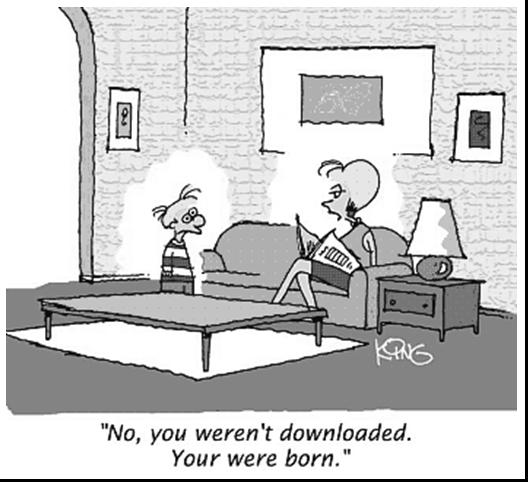
\includegraphics[width=.5\textwidth]{fig1.jpg}
\caption{A typical figure}
\label{fig:exampleFig1}
\end{figure}

\begin{figure}[ht]
\centering
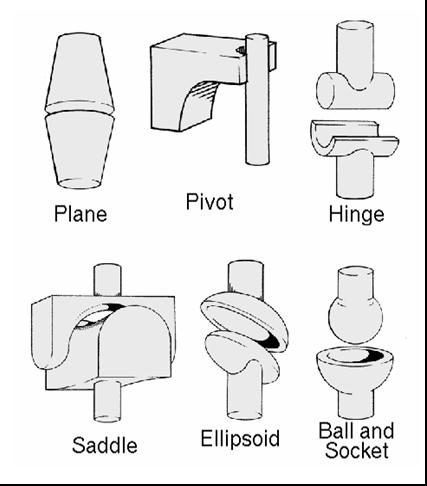
\includegraphics[width=.3\textwidth]{fig2.jpg}
\caption{This figure is an example of a figure caption taking more than one
  line and justified considering margins mentioned in Section~\ref{sec:figs}.}
\label{fig:exampleFig2}
\end{figure}

In tables, try to avoid the use of colored or shaded backgrounds, and avoid
thick, doubled, or unnecessary framing lines. When reporting empirical data,
do not use more decimal digits than warranted by their precision and
reproducibility. Table caption must be placed before the table (see Table 1)
and the font used must also be Helvetica, 10 point, boldface, with 6 points of
space before and after each caption.

\begin{table}[ht]
\centering
\caption{Variables to be considered on the evaluation of interaction
  techniques}
\label{tab:exTable1}
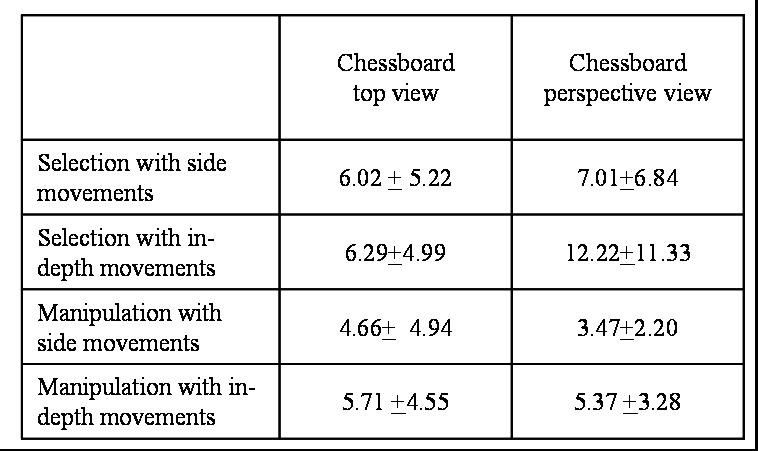
\includegraphics[width=.7\textwidth]{table.jpg}
\end{table}

\section{Images}

All images and illustrations should be in black-and-white, or gray tones,
excepting for the papers that will be electronically available (on CD-ROMs,
internet, etc.). The image resolution on paper should be about 600 dpi for
black-and-white images, and 150-300 dpi for grayscale images.  Do not include
images with excessive resolution, as they may take hours to print, without any
visible difference in the result. 

\section{References}

Bibliographic references must be unambiguous and uniform.  We recommend giving
the author names references in brackets, e.g. \cite{knuth:84},
\cite{boulic:91}, and \cite{smith:99}.

The references must be listed using 12 point font size, with 6 points of space
before each reference. The first line of each reference should not be
indented, while the subsequent should be indented by 0.5 cm.

\bibliographystyle{sbc}
\bibliography{sbc-template}

\end{document}
